\documentclass{standalone}

\AtBeginDocument{\renewcommand{\AtBeginDocument}[1]{}}
\usepackage{siunitx}

\usepackage{pgfplots}
\pgfplotsset{compat=newest}

\begin{document}
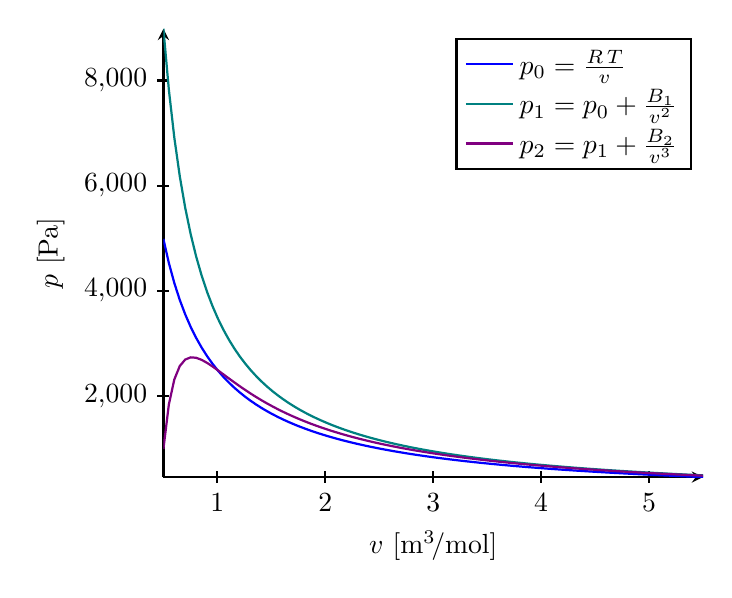
\begin{tikzpicture}

  \def\gasconstant{8.31}\def\temperature{300}
  \def\alphaCoef{10^(-3)}\def\betaCoef{10^(-5)}

  % \def\Bone{(\betaCoef*\gasconstant*\temperature - \alphaCoef)}
  % \def\Btwo{(\betaCoef^2*\gasconstant*\temperature - \alphaCoef*\betaCoef + \alphaCoef^2/(2*\gasconstant*\temperature))}
  \def\Bone{1000}
  \def\Btwo{-1000}

  \def\pzero{\gasconstant*\temperature/x}
  \def\pone{\pzero + \Bone/x^2}
  \def\ptwo{\pone + \Btwo/x^3}

  \begin{axis}[
    axis lines=left,
    samples=100,
    domain=0.5:5.5,
    xlabel={$v$ [\si[per-mode=symbol]{\meter\cubed\per\mol}]},
        ylabel={$p$ [\si{\pascal}]},
        every tick/.style={thick},
        thick]

    % p_0
    \addplot[color=blue]{\pzero};
    \addlegendentry[right]{$p_0 = \frac{R \, T}{v}$}

    % p_1
    \addplot[color=teal]{\pone};
    \addlegendentry[right]{$p_1 = p_0 + \frac{B_1}{v^2}$}

    % p_2
    \addplot[color=violet]{\ptwo};
    \addlegendentry[right]{$p_2 = p_1 + \frac{B_2}{v^3}$}

  \end{axis}
\end{tikzpicture}
\end{document}
